% Template for ICASSP-2019 paper; to be used with:
%          spconf.sty  - ICASSP/ICIP LaTeX style file, and
%          IEEEbib.bst - IEEE bibliography style file.
% --------------------------------------------------------------------------
\documentclass{article}
\usepackage{spconf,amsmath,graphicx}
\usepackage{color,amsfonts}

\usepackage{tabularx}
%\usepackage{caption}
%\captionsetup[table]{skip=2pt}

% Example definitions.
% --------------------
\def\x{{\mathbf x}}
\def\L{{\cal L}}

% Title.
% ------
\title{Nonparallel Emotional Speech Conversion}
%
% Single address.
% ---------------
%\name{Author(s) Name(s)\thanks{Thanks to XYZ agency for funding.}}
%\address{Author Affiliation(s)}
%
% For example:
% ------------
%\address{School\\
%	Department\\
%	Address}
%
% Two addresses (uncomment and modify for two-address case).
% ----------------------------------------------------------
%\twoauthors
%  {A. Author-one, B. Author-two\sthanks{Thanks to XYZ agency for funding.}}
%	{School A-B\\
%	Department A-B\\
%	Address A-B}
%  {C. Author-three, D. Author-four\sthanks{The fourth author performed the work
%	while at ...}}
%	{School C-D\\
%	Department C-D\\
%	Address C-D}
%

\name{Jian Gao $^{\star}$ \qquad Deep Chakraborty $^{\dagger}$ \qquad Olaitan Olaleye $^{\ddagger}$}
\address{$^{\star}$ Department of Computer Science and Engineering, New York University, USA \\ $^{\dagger}$ College of Information and Computer Sciences, University of Massachusetts Amherst, USA \\ $^{\ddagger}$ Signify (formerly Philips Lighting) Research, North America, USA \\
%{\small \tt jg4631@nyu.edu, dchakraborty@cs.umass.edu, olaitan.olaleye@signify.com}
}


\begin{document}
%\ninept
%
\maketitle
%
\begin{abstract}
We propose a nonparallel data-driven emotional speech conversion method. It enables the transfer of emotion-related characteristics of a speech signal while preserving the speaker's identity and linguistic content. Most existing approaches require parallel data and time alignment, which is not available in most real applications. We achieve nonparallel training based on an unsupervised style transfer technique, which learns a translation model between two distributions instead of a deterministic one-to-one mapping between paired examples. The conversion model consists of an encoder and a decoder for each emotion domain. We assume that the speech signal can be decomposed into an emotion-invariant content code and an emotion-related style code in latent space. Emotion conversion is performed by extracting and recombining the content code of the source speech and the style code of the target emotion. We tested our method on a nonparallel corpora with four emotions. Both subjective and objective evaluations show the effectiveness of our approach.
%This model consists of an autoencoder with a generative adversarial network and is trained with weak cycle consistency loss, adversarial loss, and reconstruction loss
\end{abstract}

%
\begin{keywords}
Emotional Speech Conversion, Non-parallel training, Style Transfer, Autoencoder, GANs
\end{keywords}
%



\section{Introduction}
\label{sec:intro}
Voice transformation (VT) is a technique to modify some properties of human speech while preserving its linguistic information. VT can be applied to change the speaker identity, i.e., voice conversion (VC) \cite{mohammadi2017overview}, or to transform the speaking style of a speaker, such as emotion and accent conversion \cite{zhao2018accent}. In this work, we will focus on emotion voice transformation. The goal is to change emotion-related characteristics of a speech signal while preserving its linguistic content and speaker identity. Emotion conversion techniques can be applied to various tasks, such as hiding negative emotions for customer service agents, helping film dubbing, and creating more expressive voice messages on social media.

%{\color{blue}Numerous use-cases exist for this solution including customer service representative conversation masking, financial earnings report conference calls emotion masking, conference room solutions or Instagram-like emotion-filters for speech in social media applications. \textbf{shorter?}}.

Traditional VC approaches cannot be applied directly because they change speaker identity by assuming pronunciation and intonation to be a part of the speaker-independent information. Since the speaker's emotion is mainly conveyed by prosodic aspects, some studies have focused on modelling prosodic features such as pitch, tempo, and volume \cite{wang2012emotional,wang2014multi}. In \cite{xue2018voice}, a rule-based emotional voice conversion system was proposed. It modifies prosody-related acoustic features of neutral speech to generate different types of emotions. A speech analysis-synthesis tool STRAIGHT \cite{kawahara1999restructuring} was used to extract fundamental frequency ($F_0$) and power envelope from raw audio. These features were parameterized and modified based on Fujisaki model \cite{fujisaki1984analysis} and target prediction model \cite{xue2016study}. The converted features were then fed back into STRAIGHT to re-synthesize speech waveforms with desired emotions. However, this method requires temporal aligned parallel data that is difficult to obtain in real applications; and the accurate time alignment needs manual segmentation of the speech signal at phoneme level, which is very time consuming.
%Thus this method has limitations in real-world situations.
%The manual interaction and calibration is also very time consuming.
%On the other side, automatic time alignment algorithm like dynamic time warping (DTW) may cause performance degradation due to mismatching.
% time consuming and tedious task

%it's harder to get parallel emotional speech corpora (dataset XXX) than VC.
%need professional actors, since in normal life, it's rare to find angry sentences pronounced in a happy style
To address these issues, we propose a nonparallel training method. Instead of learning one-to-one mapping between paired emotional utterances $(x_1, x_2)$, we switch to training a conversion model between two emotional domains $(\mathcal{X}_1, \mathcal{X}_2)$.

Inspired by disentangled representation learning in image style transfer \cite{gatys2016image}, we assume that each speech signal $x_i \in \mathcal{X}_i$ can be decomposed into a content code $c \in \mathcal{C}$ that represents emotion-invariant information and a style code $s_i \in \mathcal{S}_i$ that represents emotion-dependent information. $\mathcal{C}$ is shared across domains and contains the information we want to preserve. $\mathcal{S}_i$ is domain-specific and contains the information we want to change. In conversion stage, we extract content code of the source speech and recombine it with style code of the target emotion. A generative adversarial network (GAN) \cite{goodfellow2014generative} is added to improve the quality of converted speech. Our approach is nonparallel, text-independent, and does not rely on any manual operation.
%It can be trained on a small amount of utterances ($\sim$ 8 min per emotion).

%We employ gated convolutional neural networks (CNNs) ~\cite{dauphin2017language} to model the speech representations. This allows the autoencoder to capture the long-range dependencies in speech. The conversion model is trained with a weak cycle consistency loss ~\cite{Zhu_2017_ICCV, huang2018multimodal}, which helps to create pseudo pairs from nonparallel data. And and keep it indistinguishable from the real ones.

We evaluated our approach on IEMOCAP \cite{busso2008iemocap} for four emotions: angry, happy, neutral, sad,  which are widely studied in emotion speech analysis literatures.
%It is a nonparallel dataset widely used in emotional speech recognition and analysis.
An objective evaluation showed that our model can modify the speech to significantly increase the percentage of desired emotions. A subjective evaluation on Amazon MTurk showed that the converted speech had good quality and preserved the speaker identity.

The rest of the paper is organized as follows: Section \ref{sec:related} presents the relation to prior work. Section \ref{sec:method} gives a detailed description of our model. Experiment and evaluation results are reported in Section \ref{sec:exp}. Finally, we conclude in Section \ref{sec:con}.

%reviews existing work that are most closely related to our approach
% pairwise transformation function

\section{Related Work}
\label{sec:related}

\subsection{Emotion-related features}
Previous emotion conversion methods directly modify parameterized prosody-related features that convey emotions. ~\cite{kawanami2003gmm} first proposed to use Gaussian mixture models (GMM) for spectrum transformation.
%[12] introduced a data-driven emotion conversion system that combines independent parameter transformation techniques including HMM-based $F_0$ generation, $F_0$ segment selection, duration conversion and GMM-based spectral conversion. However, it requires large amounts of parallel data.
A recent work ~\cite{xue2018voice} explored four types of acoustic features: $F_0$ contour, spectral sequence, duration and power envelope, and investigated their impact on emotional speech synthesis
% by controlled feature replacement.
The authors found that $F_0$ and spectral sequence are the dominant factors in emotion conversion, while power envelope and duration alone has little influence. They further claimed that all emotions can be synthesized by modifying the spectral sequence, but did not provide a method to do it. In this paper, we focus on learning the conversion models for $F_0$ and spectral sequence.
%Since changing duration and power envelope requires manually segmenting the phoneme boundaries of vowels and consonants, we leave it for future work.

\subsection{Nonparallel training approaches}
%In parallel setting, the training data is limited to a small amount of predefined sentences, which may impair the generalization ability.
%It is a time consuming and painstaking task to collect parallel data. Training on well-aligned parallel data is easy, but collecting such data is hard.
Parallel data means utterances with the same linguistic content but varying in aspects to be studied. Since parallel data is hard to collect, nonparallel approaches have been developed. Some borrow ideas from image-to-image translation and create models suitable for speech, such as VC-VAW-GAN \cite{hsu2017voice} and VC-CycleGAN \cite{fang2018high}. Another trend is based on WaveNet \cite{van2016wavenet}. Although it can train directly on raw audio without feature extraction, the huge amount of computation resources and training data required is not affordable for most users.

%Our approach only needs a small amount of training data ($\sim$ 8 min per emotion), and does not rely on any transcripts, manual operation, or preprocessing step.
%Our method differs in that; external data

\subsection{Disentangled representation learning}
Our work draws inspiration from recent studies in image style transfer. A basic idea is to find disentangled representations that can independently model image content and style. It is claimed in ~\cite{gatys2016image} that Convolutional Neural Network (CNN) is an ideal representation to factorize semantic content and artistic style. They introduced a method to separate and recombine content and style of natural images by matching feature correlations in different convolutional layers. For us, the task is to find disentangled representations for speech signal that can split emotion from speaker identity and linguistic content.



\section{Method}
\label{sec:method}

\subsection{Assumptions}
%Emotions are nonlinguistic information not generally controlled by speakers.
The research on human emotion expression and perception has two major conclusions.
First, human emotion perception is a multi-layered process. \cite{huang2008three} figured out that humans do not perceive emotion directly from acoustic features, but through an intermediate layer of semantic primitives. They introduced a three-layered model and learnt the connections by a fuzzy inference system. Some researchers found that adding middle layers can improve emotion recognition accuracy. Based on this finding, we suggest to use multilayer perceptrons (MLP) to extract emotion-related information in speech signals.

Second, the emotion generation process of human speech follows the opposite direction of emotion perception. This means the encoding process of the speaker is the inverse operation of the decoding process of the listener. We assume that emotion speech generation and perception share the same representation methodology. This means the encoder and decoder are inverse operations with mirror structures.

Let $x_1 \in \mathcal{X}_1$ and $x_2 \in \mathcal{X}_2$ be utterances drawn from two different emotional categories. Our goal is to learn a mapping between two distributions $p(x_1)$ and $p(x_2)$. Since the joint distribution $p(x_1, x_2)$ is unknown for nonparallel data, the conversion models $p(x_1|x_2)$ and $p(x_2|x_1)$ cannot be directly estimated. To solve this problem, we make two assumptions: \\
(i). The speech signal can be decomposed into an emotion-invariant content code and an emotion-dependent style code; \\
(ii). The encoder $E$ and decoder $G$ are inverse functions.


\subsection{Model}
Fig. \ref{autoencoder} shows the generative model of speech with a partially shared latent space. A pair of corresponding speech $(x_1, x_2)$ is assumed to have a shared latent code $c \in \mathcal{C}$ and emotion-related style codes $s_1 \in \mathcal{S}_1, s_2 \in \mathcal{S}_2$. For any emotional speech $x_i$, we have a deterministic decoder $x_i = G_i(c_i,s_i)$ and its inverse encoders $c_i = E_i^c(x_i)$, $s_i = E_i^s(x_i)$. To convert emotion, we just extract and recombine the content code of the source speech with the style code of the target emotion.
\begin{equation}
\begin{aligned}
x_{1\leftarrow2}' = G_1(c_2, s_1) = G_1(E_2^c(x_2), s_1) \\
x_{2\leftarrow1}' = G_2(c_1, s_2) = G_2(E_1^c(x_1), s_2)
\end{aligned}
\end{equation}
It should be noted that the style code $s_i$ is not inferred from one utterance, but learnt from the entire emotion domain. This is because the emotion style from a single utterance is ambiguous and may not capture the general characteristics of the target emotion. It makes our assumption slightly different from the cycle consistent constraint ~\cite{Zhu_2017_ICCV}, which assumes that an example converted to another domain and converted back should remain the same as the original, i.e., $x_{1\leftarrow2\leftarrow1}'' = x_1$. Instead, we apply a semi-cycle consistency in the latent space by assuming that $E_1^c(x_{1\leftarrow2}') = c_1$ and $E_1^s(x_{1\leftarrow2}') = s_1$.

\begin{figure}[htb]
\center
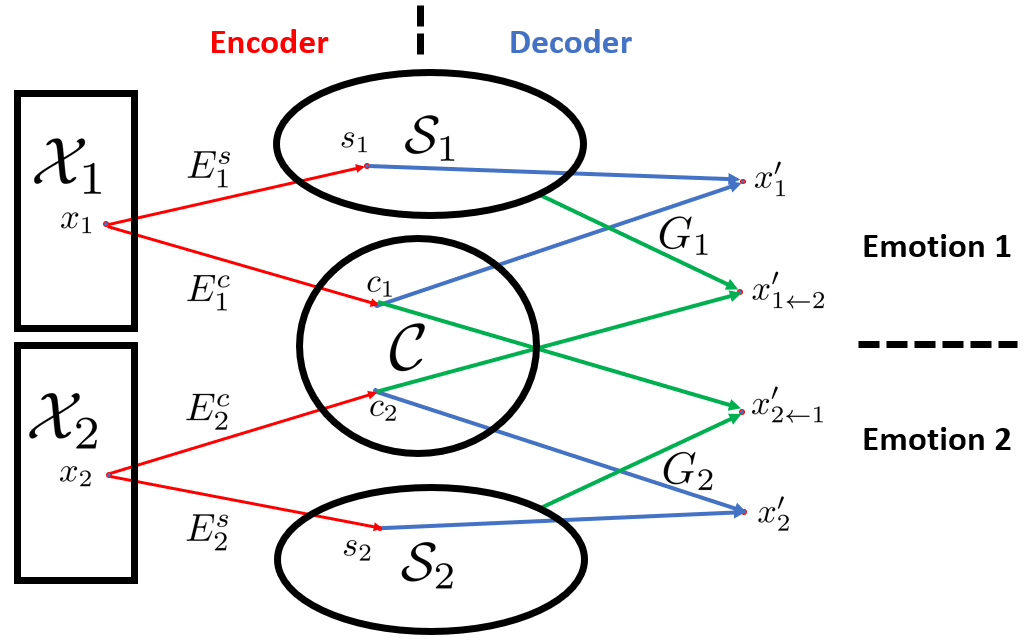
\includegraphics[width=0.4\textwidth]{FIG/autoencoder}
\caption{Speech autoencoder model with partially shared latent space. Speech with emotion $i$ is decomposed into an emotion-specific space $\mathcal{S}_i$ and a shared content space $\mathcal{C}$. Corresponding speech $(x_1,x_2)$ are encoded to the same content code $c$.
%Emotion conversion is obtained by recombining the content code of the input utterance and the style code randomly sampled from the target emotion space.
}
\label{autoencoder}
\end{figure}


% ignore the treasures in computer music before the age of deep learning.
Traditional emotional speech analysis mainly focuses on four types of acoustic features: fundamental frequency ($F_0$), spectral sequence, time duration and energy envelope. It was found in ~\cite{xue2018voice} that only $F_0$ and spectral sequence have significant influence, while the other two require manual segmentation and have little impact on changing emotions. Therefore we focus on learning the conversion model for $F_0$ and spectral sequence. Fig. \ref{model} shows an overview of our nonparallel emotional speech conversion system. The features are extracted and recombined by WORLD \cite{morise2016world} and converted separately. We modify $F_0$ by linear transform to match statistics of the fundamental frequencies in the target emotion domain. The conversion is performed by log Gaussian normalization
\begin{equation}
f_2 = \exp((\log f_1 - \mu_1)\cdot\frac{\sigma_2}{\sigma_1} + \mu_2)
\label{eq:f0}
\end{equation}
where $\mu_i, \sigma_i$ are the mean and variance obtained from the source and target emotion set. Aperiodicity (AP) is mapped directly since it does not contain emotion-related information.

\begin{figure}[htb]
\center
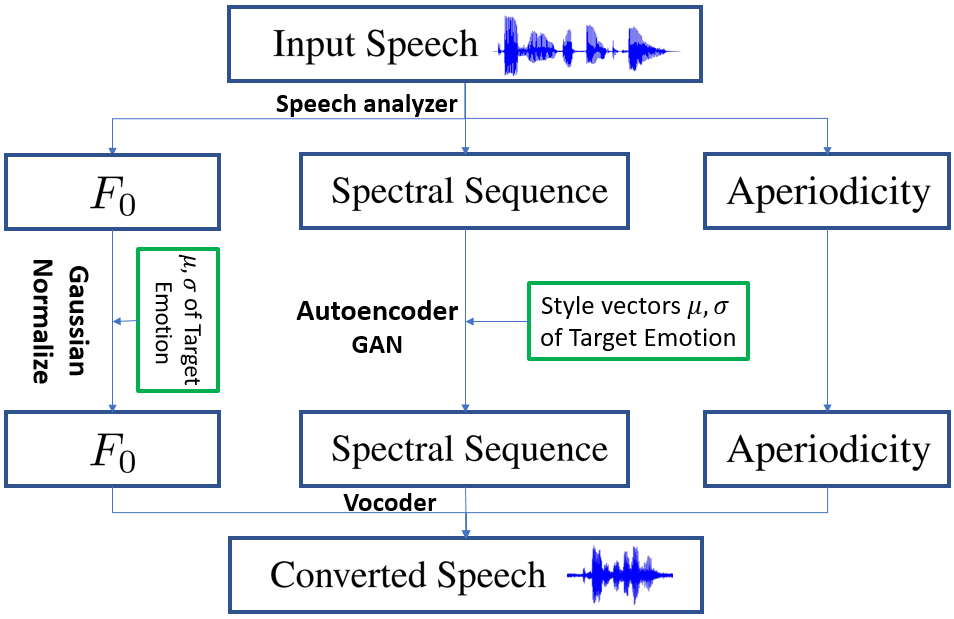
\includegraphics[width=0.4\textwidth]{FIG/model}
\caption{Overview of nonparallel emotion conversion system}
\label{model}
\end{figure}

For spectral sequence, we use low-dimensional representation in mel-cepstrum domain to reduce complexity. [28] shows that 50 MCEP coefficients are enough to synthesize full-band speech without quality degeneration. Spectra conversion is learnt by the autoencoder model in Fig. \ref{autoencoder}. The encoders and decoders are implemented with gated CNN \cite{dauphin2017language}. In addition, a GAN module is added to produce realistic spectral frames. Our model has 4 subnetworks $E^c, E^s, G, D$, in which $D$ is the discriminator in GAN to distinguish between real samples and machine-generated samples.


\subsection{Loss functions}
We jointly train the encoders, decoders and GAN's discriminators with multiple losses displayed in Fig. \ref{loss}. To keep encoder and decoder as inverse operations, we apply reconstruction loss in the direction $x_i \rightarrow (c_i, s_i) \rightarrow x_i'$. The spectral sequence should not change after encoding and decoding.
\begin{equation}
L_{recon}^{x_i} = \mathbb{E}_{x_i}(\| x_i - x_i' \|_1), \quad x_i' = G_i(E_i^c(x_i), E_i^s(x_i))
\end{equation}

\begin{figure}[htb]
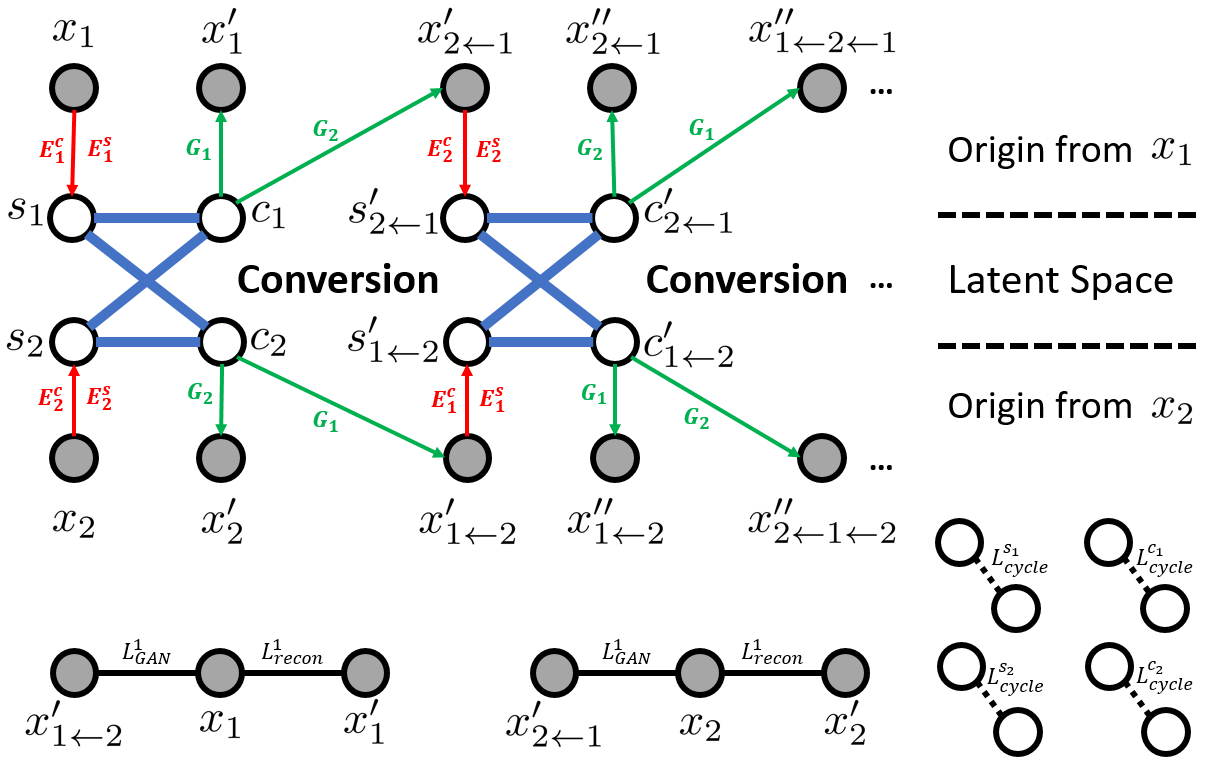
\includegraphics[width=0.48\textwidth]{FIG/loss}
\caption{Train on multiple loss functions}
\label{loss}
\end{figure}

In our model, the latent space is partially shared. Thus the cycle consistency constraint ~\cite{Zhu_2017_ICCV} is not preserved, i.e., $x_{1\leftarrow2\leftarrow1}'' \neq x_1$. We apply a semi-cycle loss in the coding direction $c_1 \rightarrow x_{2\leftarrow1}' \rightarrow c_{2\leftarrow1}'$ and $s_2 \rightarrow x_{2\leftarrow1}' \rightarrow s_{2\leftarrow1}'$.
\begin{equation}
\begin{aligned}
L_{cycle}^{c_1} = \mathbb{E}_{c_1, s_2} (\| c_1 - c_{2\leftarrow1}' \|_1), \quad c_{2\leftarrow1}'=E_2^c(x_{2\leftarrow1}') \\
L_{cycle}^{s_2} = \mathbb{E}_{c_1, s_2} (\| s_2 - s_{2\leftarrow1}' \|_1), \quad s_{2\leftarrow1}'=E_2^s(x_{2\leftarrow1}')
\end{aligned}
\end{equation}
Moreover, we add a GAN module to improve the speech quality. The converted samples should be indistinguishable from the real samples in the target emotion domain. GAN loss is computed between $x_{i\leftarrow j}'$ and $x_i$, $(i \neq j)$.
\begin{equation}
L_{GAN}^i = \mathbb{E}_{c_j, s_i}[\log(1-D_i(x_{i\leftarrow j}'))] + \mathbb{E}_{x_i}[\log D_i(x_i)]
\end{equation}
The full loss is the weighted sum of $L_{recon}$, $L_{cycle}$, $L_{GAN}$.
\begin{equation}
\begin{aligned}
\min_{E_1^c,E_1^s,E_2^c,E_2^s, G_1,G_2}\max_{D_1,D_2} L(E_1^c, E_1^s, E_2^c, E_2^s, G_1, G_2, D_1, D_2) \\
= \lambda_s (L_{cycle}^{s_1} + L_{cycle}^{s_2}) + \lambda_c (L_{cycle}^{c_1} + L_{cycle}^{c_2}) \ \qquad \qquad \\
+ \lambda_x (L_{recon}^1 + L_{recon}^2) + \lambda_g (L_{GAN}^1 + L_{GAN}^2) \qquad \quad
\end{aligned}
\end{equation}
where $\lambda_s, \lambda_c, \lambda_x, \lambda_g$ control the weights of the components.



\begin{figure*}[t!]
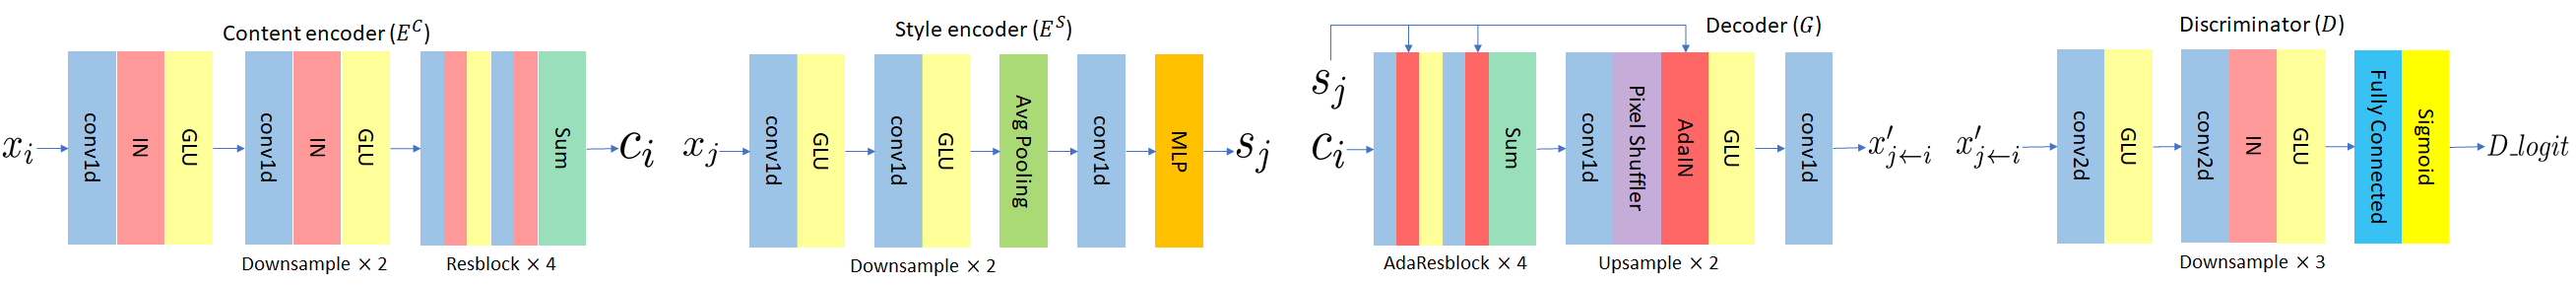
\includegraphics[width=1.0\textwidth]{FIG/NN}
\caption{The network structure of content encoder, style encoder, decoder, and GAN discriminator.}
\label{fig:NN}
\end{figure*}

\section{Experiments}
\label{sec:exp}

\subsection{Corpus}
We test the proposed method on IEMOCAP \cite{busso2008iemocap}, which is a widely used corpus for emotion recognition. To our knowledge, this is the first work to use it for emotion conversion. IEMOCAP contains scripted and improvised dialogs in five sessions; each has labeled emotional sentences pronounced by two English speakers. The emotions in scripted dialogs have strong correlation with the lingual content. Since our task is to change emotion but keep the speaker identity and linguistic content, we only use the improvised dialogs of the same speaker. We train the conversion model on four emotions: angry, happy, neutral, sad. The acoustic features $F_0$, spectral sequence and AP are extracted by WORLD \cite{morise2016world} every $5$ ms, then encoded to $24$-dimension mel-cepstral vectors of temporal size $w=128$ as the autoencoder's input.


\subsection{Network Structure}
Our network structure is illustrated in Fig. \ref{fig:NN}. The encoders and decoders are implemented with 1-dimension CNNs to capture the temporal dependencies; the GAN discriminators are implemented with 2-dimension CNNs to capture the spectra-temporal patterns. All networks are equipped with gated linear units (GLU) \cite{dauphin2017language} as activation functions. The emotion style is learnt by a $3$-linear MLP that outputs channel-wise mean and variance $\mu(s), \sigma(s)$. Then they are fed into the decoder by adding an adaptive instance normalization (AdaIN) [28] layer before activation. This mechanism is similar to the conversion model of $F_0$ in eq. (\ref{eq:f0}).
\begin{equation}
\text{AdaIN}(c,s) = \sigma(s)\Big(\frac{c-\mu(c)}{\sigma(c)}\Big) + \mu(s)
\end{equation}
We use Adam optimizer and set $\beta_1=0.5$. The learning rate is initialized as $0.0001$ and linearly decayed to $0$ from the $200K$-th iteration. We set $\lambda_s = \lambda_c = \lambda_g = 1$ and $\lambda_x=10$. For training, we randomly sample fixed length frames (128) from the input audio with $16$KHz frequency. Conversion was conducted on speech sequences with arbitrary length.


\subsection{Results}
The results were evaluated on three matrices: voice quality, emotion correctness, and the ability to keep speaker identity.

\noindent \textbf{Subjective evaluation \ } We conducted listening tests on Amazon MTurk to evaluate the converted speech \footnote{We provide converted samples at https://www.jian-gao.org/emovc}. Each example was listened by $5$ random evaluators. They were asked to manually classify the emotion, and give $1$-to-$5$ opinion scores on voice quality and the similarity with the original speaker. The mean opinion score (MOS) of the latter two metrics were listed in Fig. \ref{fig:mos}. For emotion classification, we found results consistent with the objective evaluations, therefore omitted for space constraints.

%we found consistent results with the subjective evaluations.

%The result is shown in Table \ref{tab:sub}. We observe results that are somewhat similar to the model classification results. We also qualitatively surveyed Mturk {\color{blue} workers about} speaker identity retention and over 70\% of respondents identified the generated speech as non-synthetically generated and from the same speaker \footnote{The complete survey results, survey methodology and other results are also provided at https://www.jian-gao.org/emovc}}.

\begin{figure}[htb]
\center
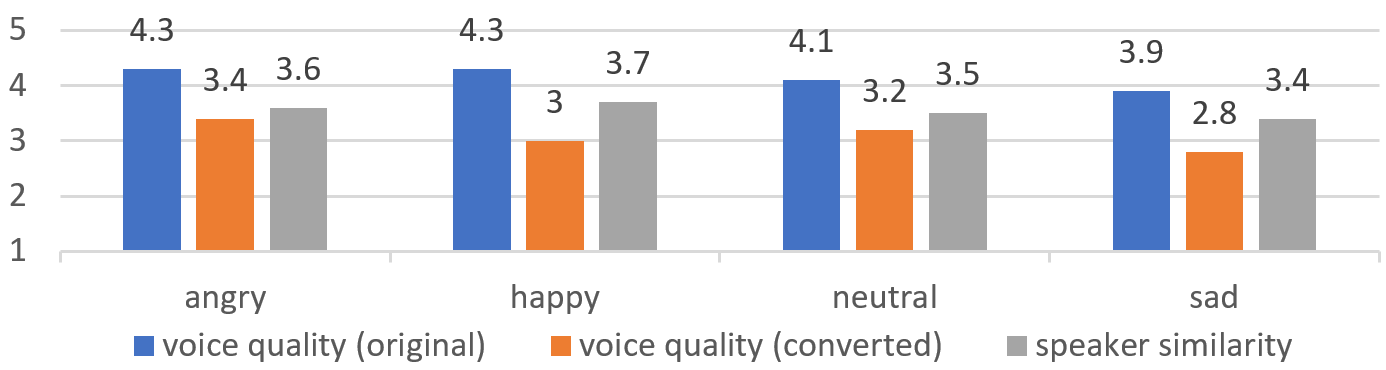
\includegraphics[width=0.45\textwidth]{FIG/MOS}
\caption{MOS for voice quality and speaker similarity}
\label{fig:mos}
\end{figure}

%\begin{table}[htb]
%\caption{MOS for voice quality and speaker similarity}
%\label{tab:mos}
%\begin{center}
%\begin{tabular}{|l|l|}
%    \hline
%    SGD 		&  $\eta = 0.1$ \\
%    \hline
%    Adam 		&  $\eta = 0.0002, \beta_1 = 0.5, \beta_2 = 0.999, \epsilon = 10^{-8}$ \\
%    \hline
%    Bregman     &  $t_0 = 0.1, t_{max} = 2.0, \Delta t=10^{-3}$ \\
%    \hline
%    SGD 		&  $\eta = 0.005$ \\
%    \hline
%    Adam 		&  $\eta = 0.0002, \beta_1 = 0.9, \beta_2 = 0.999, \epsilon = 10^{-8}$ \\
%    \hline
%    Bregman     &  $t_0 = 0.5, t_{max} = 3.0, \Delta t=10^{-4}$ \\
%    \hline
%\end{tabular}
%\end{center}
%\end{table}

%\begin{table}[ht]
%\caption{Mechanical Turk Emotion Classification Results}
%\begin{tabular}{|l|l|l|l|l|}
%\hline
%                     & \multicolumn{4}{c|}{\textbf{Predicted Class}} \\ \hline
%\textbf{IEMOCAP GT}  & Angry   & Happy   & Neutral  & Sad   \\ \hline
%Angry                & 62\%    & 15\%    & 21\%     & 2\%   \\ \hline
%Happy                & 12\%    & 51\%    & 34\%     & 2\%   \\ \hline
%Sad                  & 7\%     & 21\%    & 33\%     & 39\%  \\ \hline
%Angry to Sad         & 16\%    & 17\%    & 58\%     & 9\%   \\ \hline
%Sad to Angry         & 17\%    & 16\%    & 32\%     & 35\%  \\ \hline
%Happy to Sad         & 7\%     & 31\%    & 56\%     & 5\%   \\ \hline
%Sad to Happy         & 4\%     & 24\%    & 45\%     & 27\%  \\ \hline
%Angry to Happy       & 53\%    & 17\%    & 27\%     & 3\%   \\ \hline
%Happy to Angry       & 18\%    & 50\%    & 29\%     & 3\%   \\ \hline
%\end{tabular}
%\label{tab:subjective}
%\end{table}


\noindent \textbf{Objective evaluation \ } In addition, we applied a state-of-the-art speech emotion classifier \cite{mirsamadi2017automatic} for objective evaluation. The results listed in Table \ref{tab:emo} show that our model can effectively increase the percentage of desired emotions. Note that neutral and sad speech often get mixed up even by humans.

%{\color{blue} Overlap between neu and sad. }

%to predict the emotion in the source utterance $x_i$ and converted utterance $x_{i\leftarrow j}'$, $(i \neq j)$. The classifier consists of a Bidirectional LSTM with mean pooling over all time-steps followed by softmax over four emotion classes. {\color{blue} We evaluate the emotion in both labelled utterances from IEMOCAP and the output utterances of our model after conversion for the pairs [Angry$\rightarrow$Sad, Happy$\rightarrow$Sad and Angry$\rightarrow$Happy]. We show results in Table \ref{tab:obj}. We observe that compared to the baseline results, our approach enables emotion transfer from a source emotion towards a target emotion. For example, in the Angry to Sad emotion transfer, most of the Angry emotion is converted into a milder emotion i.e. Neutral or Sad
%Bi-LSTM Classifier

%\begin{table}[htb]
%\caption{Emotion classification by humans and machine \cite{mirsamadi2017automatic}}
%\label{tab:emo}
%\begin{center}
%\begin{tabular}{|l|l|l|l|l|}
%    \hline
%    SGD 		&  $\eta = 0.1$ \\
%    \hline
%    Adam 		&  $\eta = 0.0002, \beta_1 = 0.5, \beta_2 = 0.999, \epsilon = 10^{-8}$ \\
%    \hline
%    Bregman     &  $t_0 = 0.1, t_{max} = 2.0, \Delta t=10^{-3}$ \\
%    \hline
%    SGD 		&  $\eta = 0.005$ \\
%    \hline
%    Adam 		&  $\eta = 0.0002, \beta_1 = 0.9, \beta_2 = 0.999, \epsilon = 10^{-8}$ \\
%    \hline
%    Bregman     &  $t_0 = 0.5, t_{max} = 3.0, \Delta t=10^{-4}$ \\
%    \hline
%\end{tabular}
%\end{center}
%\end{table}
\begin{table}[htb]
\caption{Emotion classification by method in \cite{mirsamadi2017automatic}}
\resizebox{0.5\textwidth}{!}{%
\begin{tabular}{|l|l|l|l|l|}
\hline
& \multicolumn{4}{c|}{\textbf{emotion percentage \% origin (converted)}} \\ \hline
\textbf{model}   & \textbf{Angry}      & \textbf{Happy}    & \textbf{Neutral}  & \textbf{Sad}   \\ \hline
neu2ang       & \textbf{5(26)}     & 7(14)   & \textbf{19(9)}  & 70(51)   \\ \hline
ang2neu       & \textbf{84(16)}    & 5(16)   & \textbf{11(63)} & 0(5)     \\ \hline
\hline
hap2sad       & 12(7)     & \textbf{51(31)}  & 34(56) & \textbf{2(5)}     \\ \hline
sad2hap       & 7(4)      & \textbf{21(24)}  & 33(45) & \textbf{39(27)}   \\ \hline
\hline
ang2sad       & \textbf{62(16)}    & 15(17)  & 21(58)  & \textbf{2(9)}   \\ \hline
sad2ang       & \textbf{7(17)}    & 21(16)  & 33(32)  & \textbf{39(35)}   \\ \hline
\hline
ang2hap       & \textbf{72(32)}      & \textbf{8(16)}   & 10(53)    & 10(0)   \\ \hline
hap2ang       & \textbf{12(63)}      & \textbf{65(16)}    & 12(22)    & 12(0)   \\ \hline
\end{tabular}}
\label{tab:emo}
\end{table}

%\begin{table}[ht]
%\caption{Objective evaluation on Bi-Directional LSTM Classifier \cite{mirsamadi2017automatic}}
%\begin{tabular}{|l|l|l|l|l|}
%\hline
%                     & \multicolumn{4}{c|}{\textbf{Predicted Class}} \\ \hline
%\textbf{IEMOCAP GT}  & Angry   & Happy   & Neutral  & Sad   \\ \hline
%Angry                & 72\%    & 8\%     & 10\%     & 10\%  \\ \hline
%Happy                & 12\%    & 65\%    & 12\%     & 12\%  \\ \hline
%Neutral              & 7\%     & 7\%     & 35\%     & 51\%  \\ \hline
%Sad                  & 3\%     & 3\%     & 6\%      & 88\%  \\ \hline
%Angry to Sad         & 0\%     & 5\%     & 74\%     & 21\%  \\ \hline
%Sad to Angry         & 21\%    & 0\%     & 21\%     & 57\%  \\ \hline
%Happy to Sad         & 0\%     & 0\%     & 81\%     & 13\%  \\ \hline
%Sad to Happy         & 21\%    & 0\%     & 21\%     & 57\%  \\ \hline
%Angry to Happy       & 32\%    & 16\%    & 53\%     & 0\%   \\ \hline
%Happy to Angry       & 63\%    & 16\%    & 22\%     & 0\%   \\ \hline
%\end{tabular}
%\label{tab:objective}
%\end{table}





\section{Conclusion and Future work}
\label{sec:con}
We presented a nonparallel emotional speech conversion system. Objective and subjective evaluations showed that our model can successfully manipulate emotions to fool the emotion classifier as well as human listeners. As our approach does not require any paired data, transcripts or time alignment, it is easy to be applied in real-world situations. To our knowledge, this is the first work for nonparallel emotion conversion using style transfer technique. Future work is to develop a unified general model that can do multi-domain emotion conversion for unseen speakers.

%{\color{blue} One limitation is that the current model is restricted to one specific speaker.}

%$x_1, x_2, x_1', x_2'$
%$s_1, c_1, s_2, c_2$ \\
%$c_{1\leftarrow2}', s_{1\leftarrow2}', c_{2\leftarrow1}', s_{2\leftarrow1}'$ \\
%$x_{2\leftarrow1}', x_{1\leftarrow2}', x_{2\leftarrow1}'', x_{1\leftarrow2}''$ \\
%$x_{1\leftarrow2\leftarrow1}'', x_{2\leftarrow1\leftarrow2}''$
\newpage

% References should be produced using the bibtex program from suitable
% BiBTeX files (here: strings, refs, manuals). The IEEEbib.bst bibliography
% style file from IEEE produces unsorted bibliography list.
% -------------------------------------------------------------------------
\bibliographystyle{IEEEbib}
\bibliography{refs}

\end{document}


